\chapter{Metodologie e tecnologie}\label{teoria}

In questo capitolo descriverò gli strumenti utilizzati per la realizzazione ed il testing del progetto. Tra di essi mi soffermerò in particolare sul \textit{framework} \gls{spring} (e relativi moduli derivati), il broker \gls{rabbitmq} e l'architettura a microservizi dato che sono stati i principali ambiti di studio nel periodo di tirocinio.

%%%%%%%%%%  ARCHITETTURA A MICROSERVIZI %%%%%%%%%%
\section{Architettura a Microservizi}

\begin{figure}[H]
    \centering
    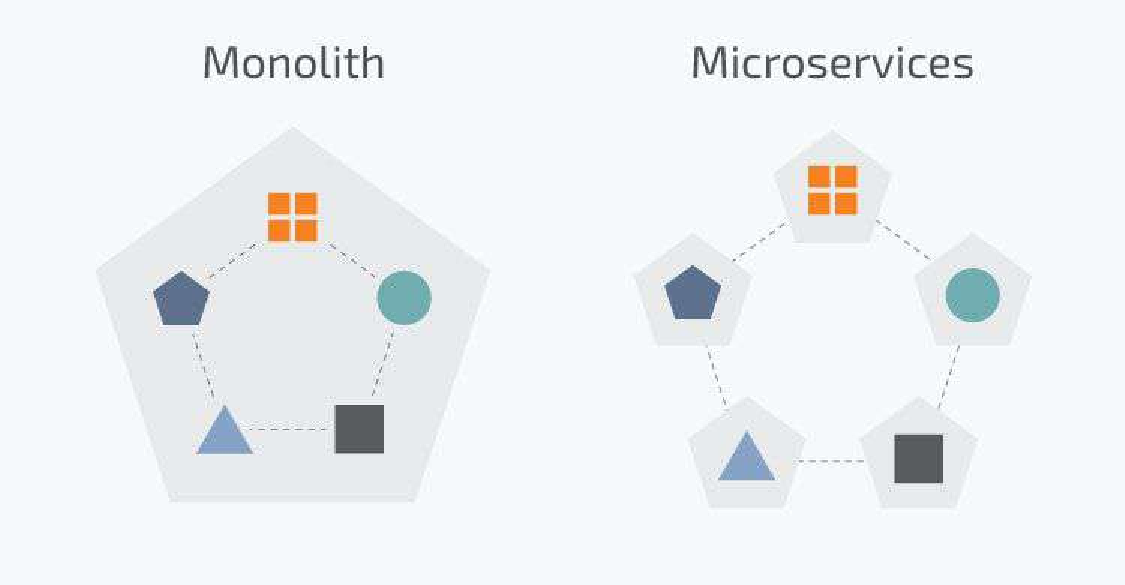
\includegraphics[width=11cm, height=6cm]{images/monoVSmicro.pdf}
    \caption{Architettura monolitica vs microservizi. Fonte: N-iX}
\end{figure}

Nel mondo della programmazione una delle nuove tendenze è l'adozione dell'architettura a microservizi per la creazione di applicazioni \cite{monomicro}. L'approccio a microservizi offre infatti vantaggi tangibili, tra cui un aumento della scalabilità, della flessibilità e dell'agilità. Molti leader tecnologici hanno effettuato con successo il passaggio dall'architettura monolitica ai microservizi, e ad ora molte aziende considerano di seguire questo esempio come il modo più efficiente per la crescita del business.\\
Dal canto suo l'approccio monolitico è un modello predefinito per la creazione di un'applicazione software. Tuttavia la sua popolarità sta diminuendo dato che questo tipo di architettura pone una serie di sfide associate, quali una grossa mole di codice, la difficoltà nell'adozione di una nuova tecnologia e dell'implementazione di modifiche.

\subsection{Monolitica vs. Microservizi}
%%%%%%%%%%  ARCHITETTURA MONOLITICA %%%%%%%%%%
\begin{flushleft}
\textbf{{\large Architettura Monolitica}}
\end{flushleft}

L'architettura monolitica è considerata la via tradizionale nella costruzione delle applicazioni. Un'applicazione monolitica è costituita da una singola ed indivisibile unità dove vengono gestite tutte le operazioni. Tra queste possiamo trovare l'interfaccia grafica atta alla comunicazione con l'utente e la comunicazione/gestione del database. Di prassi l'architettura monolitica è caratterizzata da una grande mole di codice e da mancanza di modularità. Se è necessario effettuare un aggiornamento o cambiare qualcosa, i programmatori dovranno accedere allo stesso codice, modificando l'intera applicazione.

\begin{figure}[H]
    \centering
    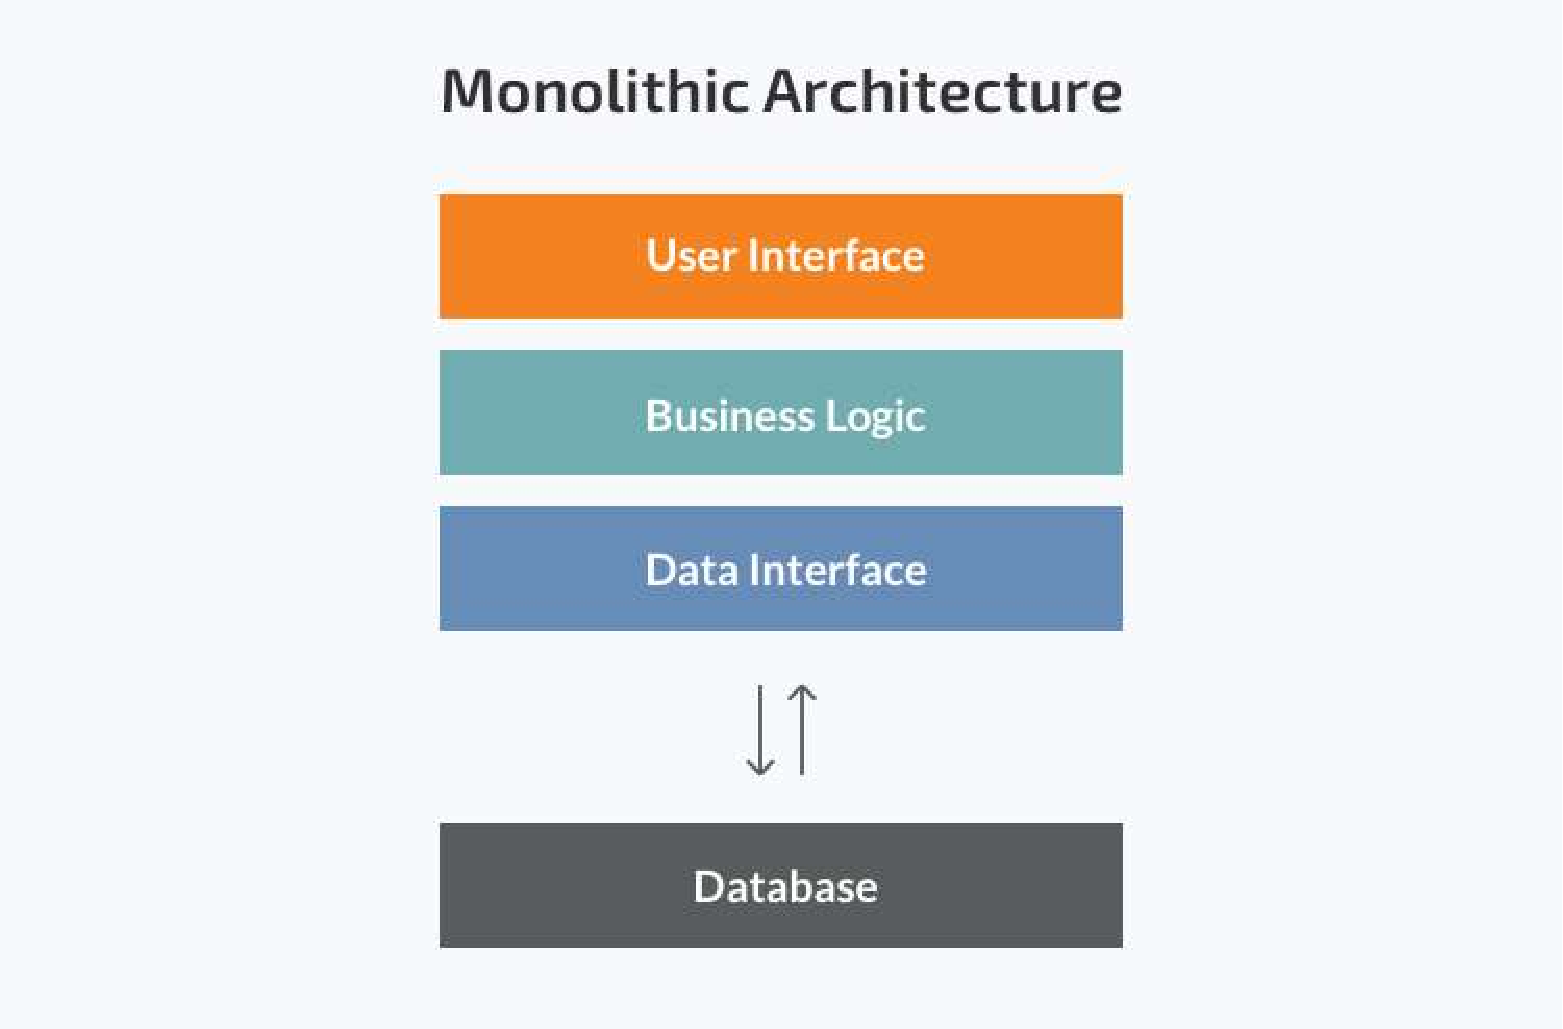
\includegraphics[width=10cm, height=6cm]{images/mono.pdf}
    \caption{Architettura monolitica. Fonte: N-iX}
\end{figure}

I punti di forza di questo tipo di architettura sono la semplicità di sviluppo, derivante dal fatto che il modello monolitico è uno standard per creare applicazioni, e di distribuzione, la riduzione dei problemi trasversali quali il \textit{logging}, il \textit{caching} ed il monitoraggio delle prestazioni. Infine il \textit{debugging} ed il \textit{testing} sono più semplici dato che riguardano una singola unità indivisibile.\\
I punti di debolezza sono principalmente legati alla gestione del codice nel tempo. Mano a mano che l'applicazione si arricchisce di nuove funzionalità diventa difficile la comprensione d'insieme.

\begin{table}[H]
    \centering
    \begin{tabular}{ |c|c| }
        \hline
        Pro & Contro \\
        \hline
        Meno problemi trasversali & Difficoltà di comprensione \\
        Semplicità debugging e testing & Difficoltà nella manutenzione \\
        Semplicità di sviluppo & Nessuna scalabilità di componenti \\
        Semplicità di distribuzione & Problematica nuove tecnologie \\
        \hline
    \end{tabular}
    \caption{Pro e contro di una architettura monolitica}
\end{table}
%%%%%%%%%%  ARCHITETTURA A MICROSERVIZI %%%%%%%%%%
\begin{flushleft}
\textbf{{\large Architettura a Microservizi}}
\end{flushleft}

Mentre un'applicazione monolitica è una singola indivisibile unità, l'architettura a microservizi suddivide l'applicazione in una raccolta di unità indipedenti più piccole. Queste unità eseguono ogni processo dell'applicazione come un servizio separato, così ognuno di questi servizi può avere una propria logica ed un proprio database.\\
All'interno di un'architettura a microservizi l'intero applicativo è suddiviso in moduli distribuiti in modo indipendente che comunicano tra loro attraverso le \Gls{api}. Ogni servizio può essere aggiornato, distribuito e ridimensionato in modo indipendente.

\begin{figure}[H]
    \centering
    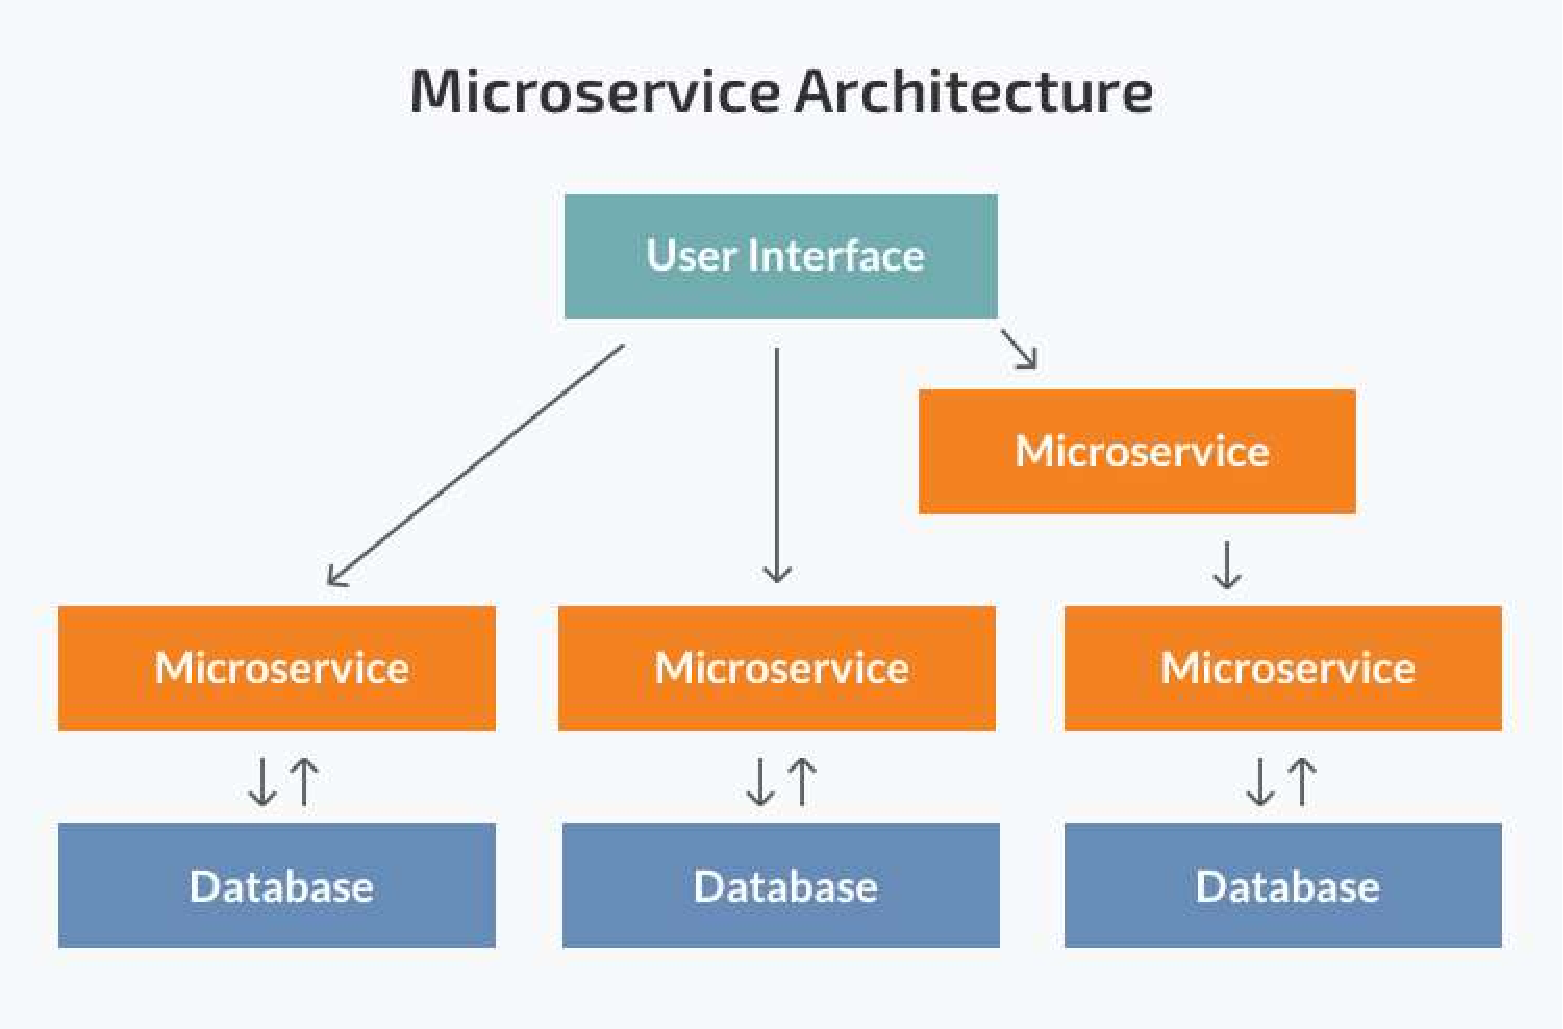
\includegraphics[width=10cm, height=6cm]{images/micro.pdf}
    \caption{Architettura a microservizi. Fonte: N-iX}
\end{figure}

I punti di forza di questo tipo di architettura sono l'indipendenza delle componenti, che permette l'implementazione e l'aggiornamento del singolo modulo; da questo deriva anche una migliore scalabilità ed il confinamento dei bug, dato che il malfunzionamento di un servizio non comporta l'interruzione di tutta l'applicazione. La divisione dei vari servizi permette una migliore e più semplice comprensione dell'applicazione ed una maggiore flessibilità nella scelta delle tecnologie.\\
I punti di debolezza riguardano la complessità di realizzazione e di \textit{testing} di un'applicazione con questa architettura, l'incremento di problemi trasversali nell'implementazione e la difficoltà di distribuzione, data l'interconnessione di più moduli indipendenti.

\begin{table}[H]
    \centering
    \begin{tabular}{ |c|c| }
        \hline
        Pro & Contro \\
        \hline
        Indipendenza delle componenti & Complessità aggiuntiva \\
        Facilità di comprensione & Difficoltà di distribuzione \\
        Migliore scalabilità & Problematiche trasversali \\
        Flessibilità nelle tecnologie & Testing difficoltoso \\
        \hline
    \end{tabular}
    \caption{Pro e contro di una architettura a microservizi}
\end{table}

\subsection{Componenti microservizi}

%%%%%%%%%%  API GATEWAY %%%%%%%%%%  
\begin{flushleft}
\textbf{{\large API Gateway}}
\end{flushleft}

\begin{figure}[H]
    \centering
    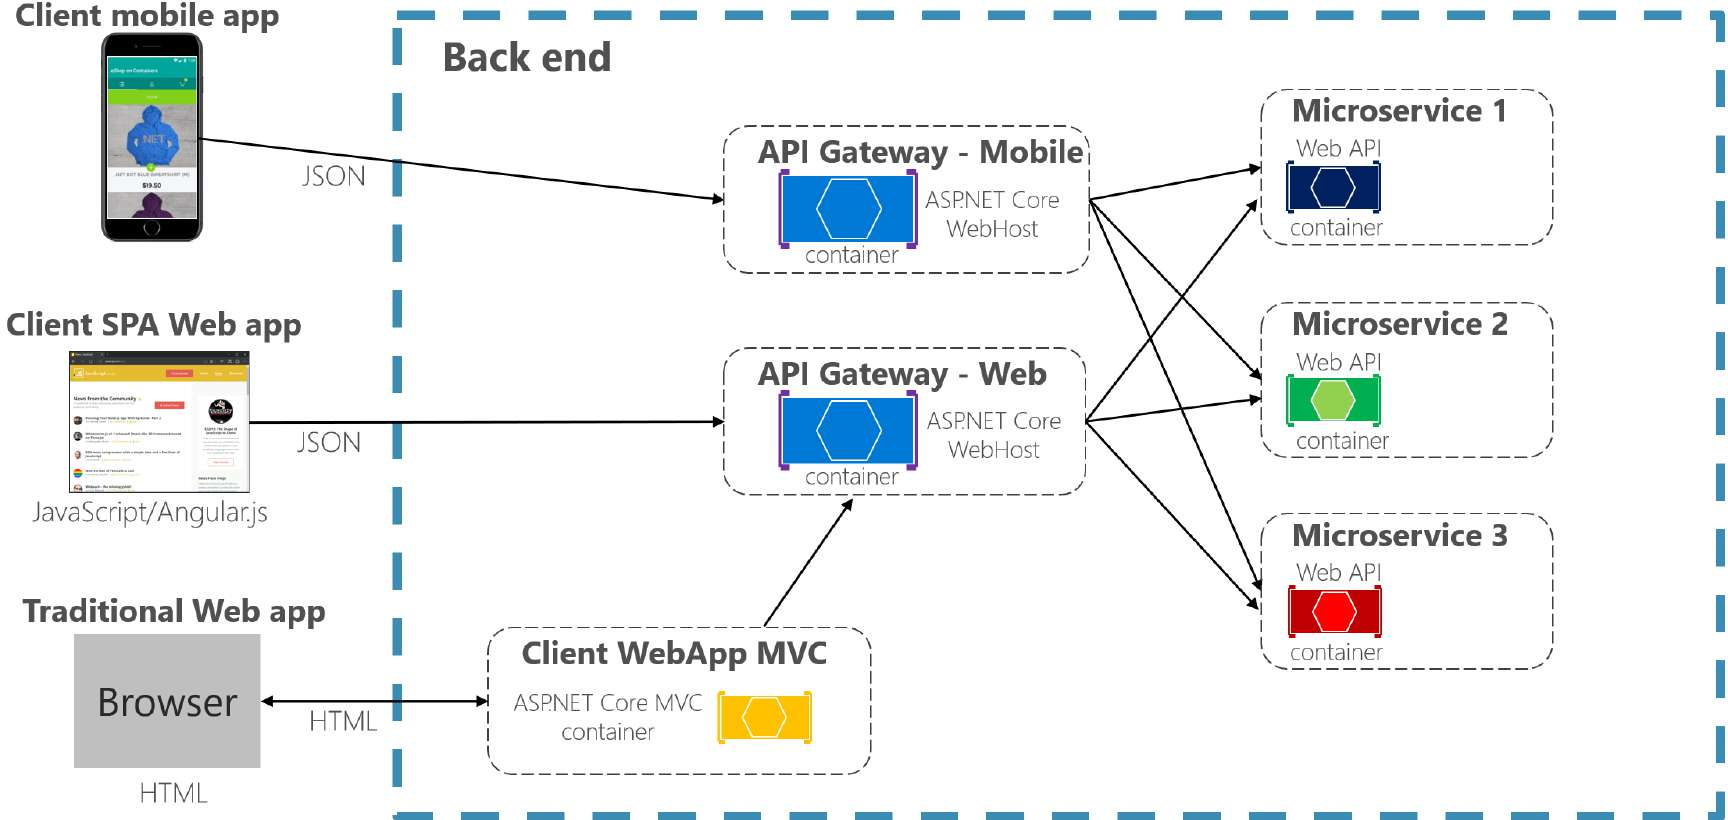
\includegraphics[width=13cm, height=8cm]{images/api-gateway.pdf}
    \caption{Servizio API Gateway. Fonte: Microsoft}
    \label{fig:apigat}
\end{figure}

%%%%%%%%%%  Circuit Breaker %%%%%%%%%%  
\begin{flushleft}
\textbf{{\large Circuit Breaker}}
\end{flushleft}

Il \textit{circuit breaker} è un modello di progettazione utilizzato nell'architettura a microservizi. I vari servizi per interagire tra loro si scambiano dati mediante richieste attraverso la rete. Durante questo scambio di informazioni è possibile che un servizio sia inattivo, per una connessione lenta, un timeout o un'indisponibilità temporanea. La soluzione migliore è far richiesta nuovamente a quel servizio, però se il problema è grave e quest'ultimo non è a disposizione per lungo tempo si può incorrere nell'eventualità in cui le chiamate a quel servizio saturino la rete, compromettendo le prestazioni e l'esperienza utente. Per ovviare a queste problematiche si utilizza il \gls{pattern} \textit{circuit breaker}: quando il numero di guasti di un servizio supera una determinata soglia l'interruttore va in stato \textit{open} per un periodo di \textit{timeout}, ritornando un errore al servizio chiamate ad ogni nuova chiamata. Trascorso questo lasso temporale l'interruttore va in stato \textit{half-open}, consentendo il passaggio di un limitato numero di richieste di richieste di test. Se queste ultime avranno esito positivo l'interruttore andrà in stato \textit{closed} e riprende il normale funzionamento. In caso contrario il periodo di \textit{timeout} ricomincia.

Un API Gateway funge da "porta d'ingresso" per accedere ai vari microservizi da un singolo punto di accesso ed anche da \textit{proxy} inverso dato che indirizza le richieste dai client ai servizi. Questo servizio sta nel mezzo tra le applicazioni ed i microservizi così non è necessario esporre i singoli applicativi, aumentando così la sicurezza. In figura \ref{fig:apigat} si nota che solitamente si utilizza più di un API Gateway così da non avere un aggregatore monolitico (che violerebbe l'autonomia dei microservizi accoppiandoli tutti tra loro).

%%%%%%%%%%  Service Discovery e Service Registry    %%%%%%%%%%
\begin{flushleft}
\textbf{{\large Service Discovery e Service Registry}}
\end{flushleft}

\begin{figure}[H]
    \centering
    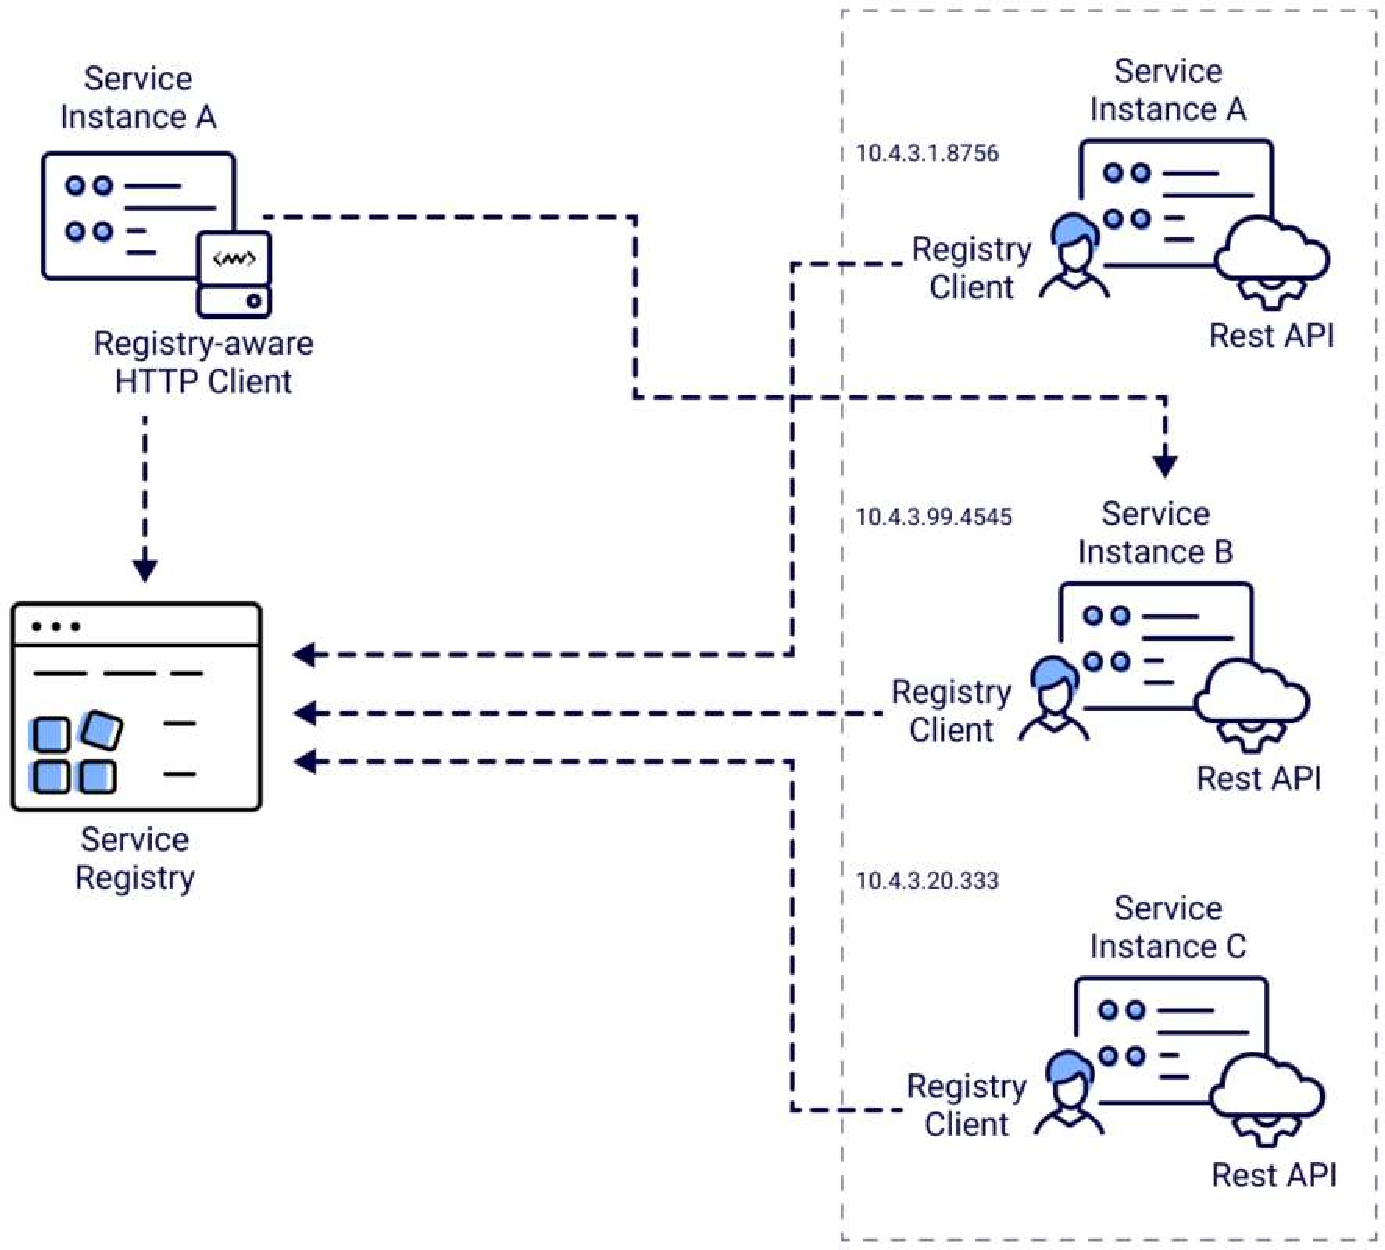
\includegraphics[width=12cm, height=9cm]{images/service-discovery.pdf}
    \caption{Schema del Service Discovery. Fonte: Middleware}
    \label{fig:servdisc}
\end{figure}

Il \textit{service discovery} è un protocollo di rete utilizzato per la rilevazione automatica di servizi e dispositivi in rete. In figura \ref{fig:servdisc} è rappresentato un \textit{service discovery} lato client come quello utilizzato nel progetto; in questo tipo di servizio il client deve ricercare il \textit{service registry} per poter individuare un servizio. Quindi il client seleziona un'istanza del servizio libera mediante un algoritmo di bilanciamento del carico.\\
Il \textit{service registry} è una componente fondamentale del \textit{service discovery}. Esso è costituito da un database contenente le locazioni di tutte le istanze dei servizi disponibili. I client possono salvare le locazioni ottenute dal \textit{service registry} nella cache, ma non devono appoggiarsi ai dati ottenuti per troppo tempo dato che quelle informazioni possono diventare velocemente obsolete.

%%%%%%%%%%  SPRING  %%%%%%%%%%
\section{Spring}\label{spring}
\Gls{spring} è un framework open source per lo sviluppo di applicazioni su piattaforma Java. Ad esso sono associati tanti altri progetti, modulari, che ne completano le funzionalità. Questi hanno nomi composti, come \textit{Spring Boot}, \textit{Spring Data} o \textit{Spring Security}. Seguirà ora un elenco dei componenti di questo framework da me utilizzati.

\begin{itemize}
    \item \textbf{Spring Boot}: questo modulo permette la creazione di una applicazione utilizzante il \textit{framework} \Gls{spring} pronta all'uso. Mediante \textit{Spring Inizializr}, \textit{Spring Boot} imposta i parametri dell'applicativo da creare (quali nome del progetto, il linguaggio utilizzato, i metadata del progetto ed il packaging) ed aiuta ad aggiungere le dipendenze necessarie tramite un checkbox.
    \item \textbf{Spring Data REST}: questo modulo permette la gestione dell'applicazione mediante chiamate \acrshort{rest} e la navigazione attraverso link.
    \item \textbf{Spring Data JPA}: questo modulo semplifica la comunicazione col database da parte dell'applicazione mediante \Gls{jpa}. Permette l'esecuzione di query, nonché l'impaginazione ed il controllo dei dati.
    \item \textbf{Spring REST Docs}: questo modulo è utile per la scrittura della documentazione progettuale e durante la fase testing. Utilizzando Postman \ref{postman}, mediante la chiamata GET \texttt{http://localhost:808x/v3/api-docs} (\textbf{x} indica un numero da 0 a 5, in base al microservizio da testare), si ha a disposizione una descrizione dei campi necessari per poter effettuare una chiamata POST o SET a quel microservizio.
    \item \textbf{Spring AMQP}: questo modulo è necessario per la corretta comunicazione dei microservizi col broker. Permette di inviare e ricevere messaggi e la dichiarazione di nuove \textit{queue}, \textit{exchange} e \textit{bindings}.
    \item \textbf{Spring Cloud Circuit Breaker}: questo modulo fornisce un'astrazione tra le diverse implementazioni dei \textit{circuit breaker}.
    \item \textbf{Spring Cloud Gateway}: questo modulo permette la creazione di un \acrshort{api} Gateway che fornisce un semplice ma efficace modo per instradare le chiamate dell'utente ai vari microservizi.
    \item \textbf{Spring Cloud Netflix}: questo modulo introduce nel progetto il \textit{service discovery} Eureka
    \item \textbf{Spring Security}: questo modulo è un framework di autenticazione e controllo accessi potente e altamente personalizzabile. È lo standard de facto per la protezione delle applicazioni basate su Spring.
\end{itemize}
%%%%%%%%%%  RABBITMQ    %%%%%%%%%%
\section{RabbitMQ}\label{rabbitmq}

\Gls{rabbitmq} è un broker di messaggi che utilizza il protocollo \acrshort{amqp} per svolgere le sue funzioni. \acrshort{amqp} è uno standard aperto che definisce un protocollo a livello applicativo per il \textit{message-oriented middleware}; questo standard è definito in modo tale da garantire funzionalità di messaggistica, accodamento e \textit{routing}, affidabilità e sicurezza \cite{amqprab}. Un broker di messaggi è una tecnologia che si fa carico della convalida, della trasformazione e del corretto indirizzamento dei messaggi. Questo strumento media la comunicazione tra le applicazioni permettendo la comunicazione attraverso lo scambio di messaggi, che possono includere qualsiasi tipo di informazione.\\
Le componenti di \Gls{rabbitmq} sono le seguenti
\begin{itemize}
    \item \textit{Publisher}: entità che comunica col broker per inviare un messaggio.
    \item \textit{Consumer}: entità che riceve un messaggio dal broker.
    \item \textit{Queue}: entità dove i messaggi sono custoditi prima dell'invio al consumer. Il legame tra \textit{queue} ed \textit{exchange} è chiamato \textit{binding}.
    \item \textit{Exchange}: entità che riceve i messaggi dal \textit{publisher} e li accoda in una o più \textit{queue}. Ci sono più tipi di \textit{exchange}.
    \begin{itemize}
        \item \textit{Fanout} accoda tutti i messaggi in tutte le \textit{queue} che conosce.
        \item \textit{Direct} accoda il messaggio alle code la cui chiave di associazione corrisponde esattamente alla \textit{routing key} del messaggio.
        \item \textit{Topic} è un insieme dei precedenti. In questo modello si instradano i messaggi verso una o più \textit{queue} in base al modello utilizzato per associare una \textit{queue} all'\textit{exchange}. Questo modello lascia maggiore libertà nello specificare le \textit{routing key} permettendo di utilizzare le \textit{wildcards} \textbf{*} per sostituire una qualsiasi parola e \textbf{\#} per sostituire 0 o più parole.
    \end{itemize}
\end{itemize}
\begin{figure}[H]
    \centering
    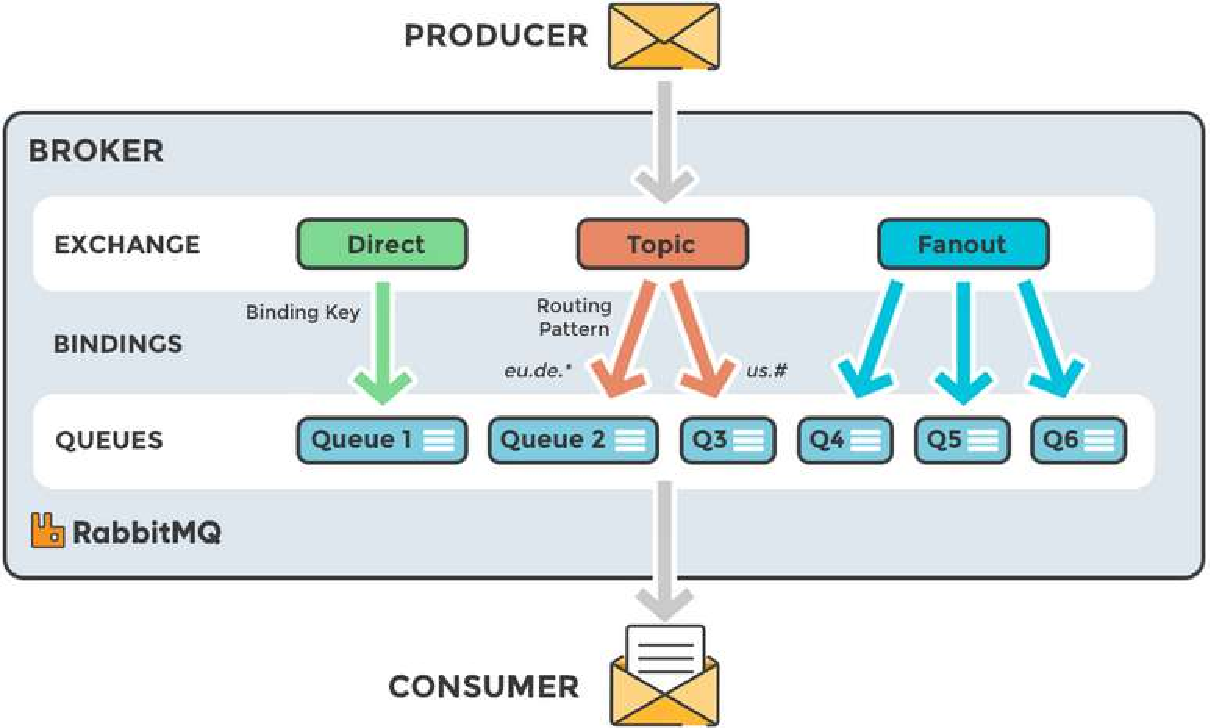
\includegraphics[width=12cm, height=6cm]{images/rabbitmq-componenti.pdf}
    \caption{Componenti del broker RabbitMQ. Fonte: RabbitMQ}
\end{figure}

Rispetto ad altri broker \Gls{rabbitmq} introduce l'\textit{queue} tra le sue componenti, e grazie a questa modifica implementa fedelmente il protocollo \acrshort{amqp}. Precedentemente vi erano solo i primi tre elementi sopracitati, con coda singola e metodo \acrshort{fifo}.\\
L'aspetto che contraddistingue \Gls{rabbitmq} rispetto ad altri broker (quali Kafka) è la capacità di lavorare molto velocemente quando le code sono quasi vuote: questo scenario è perfetto per la comunicazione tra microservizi. Inoltre la gestione delle code è più semplice, dato che il messaggio viene rimosso dalla coda una volta letto. Kafka invece è stato progettato per salvare i messaggi che arrivano per poterli leggere ed analizzare (tipicamente per il tracking degli utenti, logging) o per processarli in real-time.
%%%%%%%%%%  ALTRI SOFTWARE  %%%%%%%%%%
\section{Altri software utilizzati}\label{software}

Nell'implementazione di questo progetto sono state impiegati vari strumenti software:

\begin{itemize}
    \item \textbf{Visual Studio Code:} Visual Studio Code è un editor di codice sorgente leggero ma potente che viene eseguito sul desktop ed è disponibile per Windows, macOS e Linux. Viene fornito con il supporto integrato per JavaScript, TypeScript e Node.js e ha un ricco ecosistema di estensioni per altri linguaggi (come C++, Java, Python, PHP, Go) e runtime (come .NET e Unity) \cite{vscode}. Le estensioni utilizzate nel progetto sono state \textit{Extension Pack for Java}, \textit{Spring Boot Extension Pack}, \textit{Lombok Annotations Support for VS Code}, \textit{Docker}, \textit{Remote - Containers} e \textit{GitHub Pull Requests and Issues}.
    \item \textbf{Git:} Git è un sistema di controllo versione distribuito gratuito e open source progettato per gestire progetti sia piccoli che molto grandi con velocità ed efficienza \cite{git}. Nel progetto è stato adottato cosicché più programmatori potessero cooperare nella scrittura e nella risoluzione dei problemi.
    \item \textbf{Docker:} Docker è una piattaforma per lo sviluppo, la distribuzione e l'esecuzione di applicazioni. Consente di separare le applicazioni dall'infrastruttura in modo da poter distribuire rapidamente il software. Sfruttando le metodologie Docker si può ridurre significativamente il tempo intercorso tra la scrittura del codice e l'esecuzione in produzione \cite{docker}. Questo software è stato utilizzato per l'esecuzione di PostgreSQL e \Gls{rabbitmq} e per la creazione delle immagini dei microservizi.
    \item \textbf{Postman:}\label{postman} Postman è una piattaforma per la creazione e l'utilizzo di \Gls{api}. Postman semplifica ogni fase del ciclo di vita dell'\acrshort{api} e ottimizza la collaborazione in modo da poter creare \acrshort{api} migliori, più velocemente. La piattaforma include un set completo di strumenti che aiutano ad accelerare il ciclo di vita delle \acrshort{api}, dalla progettazione, test, documentazione e derisione alla condivisione e rilevabilità delle \acrshort{api} \cite{postman}.
    \item \textbf{DBeaver:} DBeaver è uno strumento di gestione del database universale per tutti coloro che hanno bisogno di lavorare con i dati in modo professionale. Con DBeaver si possono manipolare i dati, ad esempio in un normale foglio di calcolo, creare report analitici basati su record provenienti da diversi archivi di dati ed esportare le informazioni in un formato appropriato. Per gli utenti avanzati di database, DBeaver fornisce un potente editor SQL, numerose funzionalità di amministrazione, capacità di migrazione di dati e schemi, monitoraggio delle sessioni di connessione al database \cite{dbeaver}.
    \item \textbf{PostgreSQL:} \Gls{postgresql} è un \acrshort{dbms} ad oggetti. Il suo utilizzo nel progetto è frutto della necessità di rendere persistenti i dati, come utenti, password, lo storico delle sfide e log di sistema.
    \item \textbf{Angular:} Angular è una piattaforma per lo sviluppo di applicazioni web, basata su TypeScript. Come piattaforma, Angular include un framework basato su componenti per la creazione di applicazioni Web scalabili, una raccolta di librerie ben integrate che coprono un'ampia varietà di funzionalità, tra cui routing, gestione dei moduli, comunicazione client-server e una suite di strumenti per sviluppatori per aiutare a sviluppare, costruire, testare e aggiornare il codice.\cite{angular}
    \item \textbf{Maven}: Apache Maven è uno strumento di comprensione e gestione dei progetti software. Basato sul concetto di un modello a oggetti di progetto (\textit{POM}), Maven può gestire la creazione, il reporting e la documentazione di un progetto da un'informazione centrale \cite{maven}. Un \textit{POM} fornisce tutte le configurazioni di un singolo progetto, come per esempio il nome del progetto, la versione, il proprietario, dipendenze da altri progetti e le fasi di \textit{build} dell'applicazione.
\end{itemize}

Oltre agli strumenti sopraelencati nel progetto sono adottati anche diversi \gls{pattern}:
\begin{itemize}
    \item \textbf{Microservizi:} pattern opposto allo sviluppo monolitico in quanto ogni servizio deve poter essere sviluppato e distribuito in maniera indipendente. La comunicazione tra le varie componenti è solitamente basata su HTTP tramite chiamate REST.
    \item \textbf{Dependency injection:} Le due principali tecnologie impiegate nello sviluppo del prodotto, ovvero Angular e Spring, permettono entrambe di utilizzare il pattern \textit{dependecy injection} ovvero un \textit{design pattern} che permette di attuare l’\textit{inversion of control}. Le applicazioni Spring vengono istanziate all’interno di uno speciale container denominato \textit{IoC container} il quale si occupa di istanziare gli oggetti (\textit{beans}) dichiarati nel progetto e di reprire e iniettare tutte le dipendenze ad essi associate.
    \item \textbf{Lazy loading:} \textit{design pattern} utilizzato in \textit{Angular} che permette di caricare i moduli solo nel momento in cui effettivamente se ne ha bisogno ottenendo un guadagno in prestazioni di caricamento dell'applicazione.
\end{itemize}